\section{Contador de 8 bits con \textit{reset} asíncrono \label{sec:s3}}

\begin{center}
	\begin{minipage}{12cm}
		\begin{tcolorbox}[title=Actividad 3]
			 Codificar un contador con \textit{reset} asíncrono. Compilar y simular. Usar el visor RTL para observar como se implementa el circuito. Configurar en la tarjeta DE2-115, asignar interruptores y LED's para observar la cuenta.
		\end{tcolorbox}	
	\end{minipage}
\end{center}

La visualización RTL del contador de 8 bits con \textit{reset} asíncrono en Verilog se muestra en la \autoref{fig:counter_asyn_rst_rtl}. La implementación se hace utilizando un flip flop tipo D de 8 bits junto con una instancia de sumador de 8 bits. La señal RST se conecta al pin CLRN que sirve para limpiar el estado del contador, dicho estado se presenta en el pin SCLR, indicando que al restablecer el circuito, la salida tendrá el valor de esta terminal (para este caso, cero). La señal CLK se conecta a la terminal de reloj del flip flop y la salida Q hace una retroalimentación a la entrada D, por medio de un sumador, que incrementará el valor en 1 por cada ciclo de reloj.

Las simulaciones para el código en Verilog se visualizan en la \autoref{fig:counter_asyn_rst_wave1} y \autoref{fig:counter_asyn_rst_wave2}. Se observa que la salida Q incrementa su valor cuando hay un flanco de subida en el ciclo de reloj. La limpieza en el flip flop se da de manera asíncrona con el pin RST, ya que no depende de CLK, sino que cuando se tiene un flanco de subida en el \textit{reset}, se ajusta el valor de la salida a 0. Finalmente se ve que una vez que la cuenta llega al máximo valor posible (255 para 8 bits), hay un desbordamiento ya que se pierde el bit de acarreo, haciendo que parezca que la cuenta regresa al valor inicial.

En los Anexos se localiza la descripción del contador con \textit{reset} asíncrono. Se utilizó una lista sensible para el flanco de subida de la señal de reloj y el \textit{reset}. Dentro de esta estructura se empleó la sentencia \textit{if} para comparar el valor de RST: 
\begin{itemize}
	\item Si es 1, se restablece el valor de la salida a 0. 
	\item Si es 0, la salida adquiere el valor de D más un incremento de 1.
\end{itemize}

\begin{figure}[ht]
	\centering
	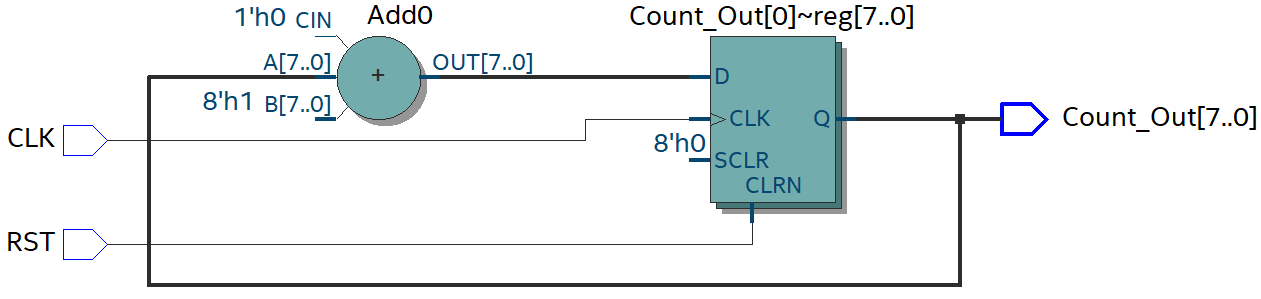
\includegraphics[scale=0.5]{Counter_Asyn_RST_RTL.png}
	\caption{Diagrama RTL del contador de 8 bits con \textit{reset} asíncrono. \label{fig:counter_asyn_rst_rtl}}
\end{figure}

\begin{figure}[ht]
	\centering
	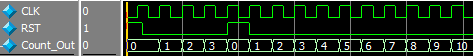
\includegraphics[scale=1.3]{Counter_Asyn_RST_Wave1.png}
	\caption{Simulación del contador de 8 bits con \textit{reset} asíncrono en el visor de formas de onda de ModelSim (Uso del \textit{reset}). \label{fig:counter_asyn_rst_wave1}}
\end{figure}

\begin{figure}[ht]
	\centering
	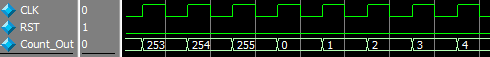
\includegraphics[scale=1.3]{Counter_Asyn_RST_Wave2.png}
	\caption{Simulación del contador de 8 bits con \textit{reset} asíncrono en el visor de formas de onda de ModelSim (Reinicio de la cuenta). \label{fig:counter_asyn_rst_wave2}}
\end{figure}